\documentclass[handout]{ximera}
\graphicspath{{./}{thePythagoreanTheorem/}{deMoivreSavesTheDay/}{complexNumbersFromDifferentAngles/}{trianglesOnACone/}{cityGeometry/}{EuclidAndGeometry/}}

\usepackage{gensymb}
\usepackage[margin=1in]{geometry}

%\usepackage{hyperref}


\usepackage{tikz}
\usepackage{tkz-euclide}
\usetkzobj{all}
\tikzstyle geometryDiagrams=[ultra thick,color=blue!50!black]
\newcommand{\tri}{\triangle}
\renewcommand{\l}{\ell}
\renewcommand{\P}{\mathcal{P}}
\newcommand{\R}{\mathbb{R}}
\newcommand{\Q}{\mathbb{Q}}

\newcommand{\Z}{\mathbb Z}
\newcommand{\N}{\mathbb N}
\newcommand{\ph}{\varphi}

\renewcommand{\vec}{\mathbf}
\renewcommand{\d}{\,d}



%% Egyptian symbols

\usepackage{multido}
\newcommand{\egmil}[1]{\multido{\i=1+1}{#1}{\includegraphics[scale=.1]{egyptian/egypt_person.pdf}\hspace{0.5mm}}}
\newcommand{\eghuntho}[1]{\multido{\i=1+1}{#1}{\includegraphics[scale=.1]{egyptian/egypt_fish.pdf}\hspace{0.5mm}}}
\newcommand{\egtentho}[1]{\multido{\i=1+1}{#1}{\includegraphics[scale=.1]{egyptian/egypt_finger.pdf}\hspace{0.5mm}}}
\newcommand{\egtho}[1]{\multido{\i=1+1}{#1}{\includegraphics[scale=.1]{egyptian/egypt_lotus.pdf}\hspace{0.5mm}}}
\newcommand{\eghun}[1]{\multido{\i=1+1}{#1}{\includegraphics[scale=.1]{egyptian/egypt_scroll.pdf}\hspace{0.5mm}}}
\newcommand{\egten}[1]{\multido{\i=1+1}{#1}{\includegraphics[scale=.1]{egyptian/egypt_heel.pdf}\hspace{0.5mm}}}
\newcommand{\egone}[1]{\multido{\i=1+1}{#1}{\includegraphics[scale=.1]{egyptian/egypt_stroke.pdf}\hspace{0.5mm}}}
\newcommand{\egyptify}[7]{
 \multido{\i=1+1}{#1}{\includegraphics[scale=.1]{egyptian/egypt_person.pdf}\hspace{0.5mm}}
 \multido{\i=1+1}{#2}{\includegraphics[scale=.1]{egyptian/egypt_fish.pdf}\hspace{0.5mm}}
 \multido{\i=1+1}{#3}{\includegraphics[scale=.1]{egyptian/egypt_finger.pdf}\hspace{0.5mm}}
 \multido{\i=1+1}{#4}{\includegraphics[scale=.1]{egyptian/egypt_lotus.pdf}\hspace{0.5mm}}
 \multido{\i=1+1}{#5}{\includegraphics[scale=.1]{egyptian/egypt_scroll.pdf}\hspace{0.5mm}}
 \multido{\i=1+1}{#6}{\includegraphics[scale=.1]{egyptian/egypt_heel.pdf}\hspace{0.5mm}}
 \multido{\i=1+1}{#7}{\includegraphics[scale=.1]{egyptian/egypt_stroke.pdf}\hspace{0.5mm}}
 \hspace{.5mm}
}




\title{It's All Greek To Me!}

\begin{document}
\begin{abstract}
    We investigate solutions to the Problems of Antiquity.
\end{abstract}
\maketitle

\begin{question}
Use your compass and straightedge to double a square with side length $s$.  That is, construct a square whose area is twice that of your original square.  Why can't we do the same for the cube?
\end{question}

Hippocrates used a ``continued mean proportional'' to double the cube.  Let's let $a$ be the side length of the original cube, and $x$ be the side length of the new, larger cube.

\begin{question}
Just to check: write an equation relating $a$ and $x$.
\end{question}

Here is an outline for how Hippocrates might have gotten his mean proportional: 
\begin{enumerate}
    \item Start with two cubes of side length $a$ next to each other.
    \item Rearrange the volume of these two cubes into a rectangular prism so that the height is unchanged, but the base rectangle has one side of length $x$.  Call the other side length $y$.
    \item Rearrange the volume again, but this time into a cube.  Use a different side as the base, and leave the ``height'' $x$ unchanged.
\end{enumerate}

\begin{question}
Draw pictures representing the geometry in the method described above.
\end{question}

\begin{question}
Write a proportion corresponding to the first rearrangement using the variables $x$, $y$, $a$, and $2a$.  Hint: we know the height of the box stays the same.  What does this mean about the area of the base?
\end{question}

\begin{question}
Write a proportion corresponding to the second rearrangement.  One of the fractions should be equal to one of the fractions from the previous question!  Then write Hippocrates' continued mean proportional by setting three fractions equal to each other.
\end{question}

\begin{question}
How is this continued mean proportional related to the equation you found in Question 2?  How might you use this information to duplicate the cube?
\end{question}

\newpage

About 420BC, Hippias invented a curve called the ``quadratrix''.  Here is its construction:
\begin{enumerate}
    \item Start with a square $ABCD$.
    \item A line segment congruent with $AB$ and coinciding with $AB$ rotates with center $A$ a quarter turn.
    \item At the same time, and at the same speed, another segment congruent with $AB$ and coinciding with $AB$ moves using straight-line motion through the square until it coincides with $CD$.
    \item Points on the quadratrix are where the two moving segments intersect.
\end{enumerate}



\begin{question}
On the square below, use a ruler and a protractor to construct at least four points on the quadratrix, and then sketch the entire curve.
\begin{image}
\begin{tikzpicture}[geometryDiagrams]
\coordinate (A) at (0,2);
\coordinate (B) at (5,2);
\coordinate (C) at (5,7);
\coordinate (D) at (0,7);
\draw (A)--(B)--(C)--(D)--cycle;
\tkzLabelPoints[above](D, C)
\tkzLabelPoints[below](A,B)

%\draw[step=.5cm] (0,0) grid (10,5);
\end{tikzpicture}
\end{image}
%\begin{image}
%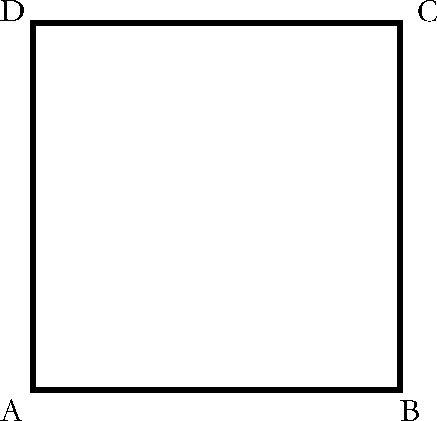
\includegraphics{squareABCD.pdf}
%\end{image}
\end{question}

\begin{question}
Let $X$ be any point on the quadratrix, and $X'$ be the point directly below $X$ on segment $AB$.  If $l$ is the length of segment $AB$ and $n$ is the length of segment $XX'$, explain why it's always true that 
\[
\frac{m\angle XAB}{m\angle DAB} = \frac{n}{l}.
\]
\end{question}

\begin{question}
Use the quadratrix to trisect an angle of $45\degree$, then an angle of $60\degree$.  Then, explain how the quadratrix can be used to trisect any angle.
\end{question}

\begin{question}
Can you use the quadratrix to square the circle?  Explain how!
\end{question}



\end{document}